% =============================================================================
% LIST OF REAL BOOK EXERCISES --- Lectures 1--4
% 24 exercises (6 per lecture: 2 foundations, 3 exam level, 1 advanced), reproduced verbatim
% under rules/00_estilo_avaliacao.md §5 and the global rule "Exercise lists built from real
% exercises". Selection taken from Listas/pratica-lecture-0{1,2,3,4}.md and re-checked against the
% rendered PDF pages. Plan: .agent/plans/lista-reais-lectures-01-04.md. No answer key.
%
% Compile (copyable PDF, global lmodern+cmap rule):
%   pdflatex lista-reais-lectures-01-04.tex   (2x)
%   pdffonts lista-reais-lectures-01-04.pdf   (all Type 1)
% =============================================================================
\documentclass[11pt,a4paper]{article}
\usepackage[utf8]{inputenc}
\usepackage[T1]{fontenc}
\usepackage{lmodern}   % Type 1 vector fonts (replaces PK bitmaps)
\usepackage{cmap}      % ToUnicode CMap -> copyable text and accents
\usepackage[english]{babel}
\usepackage{amsmath,amssymb,amsfonts,mathtools}
\usepackage[a4paper,margin=2.2cm]{geometry}
\usepackage{enumitem}
\usepackage{fancyhdr}
\usepackage{xcolor}
\usepackage{microtype}
\usepackage{booktabs}
\usepackage{graphicx}
\usepackage{array}
\usepackage{needspace}

\newcommand{\disciplina}{Economia das Organizações e dos Incentivos --- MPE Insper}
\newcommand{\listatema}{Real Book Exercises, Lectures 1--4}
\newcommand{\espacoresol}{3.5cm}   % height of the resolution space after each exercise

\pagestyle{fancy}\fancyhf{}
\lhead{\footnotesize\disciplina}
\rhead{\footnotesize \listatema}
\cfoot{\footnotesize\thepage}
\renewcommand{\headrulewidth}{0.3pt}
\setlength{\headheight}{14pt}

\setlist{topsep=2pt,itemsep=2pt}
\setlength{\parindent}{0pt}
\setlength{\parskip}{4pt}
\newcounter{questao}

% Block header: number, lecture title, coverage.
\newcommand{\bloco}[3]{\bigskip\noindent
  {\large\bfseries\color{blue!55!black}Block #1 --- #2}\hfill\textit{(#3)}\par
  \noindent\rule{\linewidth}{0.3pt}\smallskip}
% Exercise header: #1 short name, #2 level, #3 source line.
\newcommand{\exercicio}[3]{\needspace{12\baselineskip}\refstepcounter{questao}\medskip\noindent
  \textbf{Exercise \thequestao.}~\textit{#1}\hfill{\small[#2]}\par
  \noindent{\small\color{black!70}\textbf{Source.} #3}\par\smallskip}
% Material an exercise refers to, copied in under its own source line.
\newenvironment{referencia}[1]{\par\smallskip\noindent
  \begin{minipage}{\linewidth}\small\leftskip=1.2em
  \noindent\textbf{Referenced material.} {\color{black!70}\textbf{Source.} #1}\par\smallskip}%
  {\end{minipage}\par}
% Book's exercise label inside the statement, e.g. "4.5".
\newcommand{\rot}[1]{\textbf{#1}\quad}
\newcommand{\resolespaco}{\par\textit{Resolution:}\vspace{\espacoresol}\par}
% Payoff matrix: #1 row-player label, #2 column-player label, #3 inner tabular.
\newcommand{\jogo}[3]{\begin{center}\begin{tabular}{@{}r@{\hspace{6pt}}c@{}}
  & #2\\[2pt] #1 & #3\end{tabular}\end{center}}
\newcommand{\hd}[1]{\multicolumn{1}{c}{#1}}
\newenvironment{partes}{\begin{enumerate}[label=\alph*.,leftmargin=2em]}{\end{enumerate}}

% =============================================================================
\begin{document}
\begin{center}
  {\Large\bfseries \disciplina}\\[2pt]
  {\large Exercise List: \listatema}
\end{center}

{\small\noindent\textbf{How to use this list.} Every exercise below is a real exercise from one of
the course books, reproduced verbatim: the source line gives author, book, chapter, exercise,
the printed page and, in brackets, the page your PDF viewer shows for the file in
\texttt{Livros/}, and whether the source gives the answer. Muñoz-Garcia \& Toro-Gonzalez print a
worked answer right after each exercise; MWG answers are in the MWG solutions manual in
\texttt{Livros/}; Tadelis and Gibbons give no answer in the book. When an exercise refers to a
model, game or figure stated elsewhere in its book, that material is copied into the same block
under ``Referenced material'', so every exercise can be solved where it is printed. There is one
block per lecture, six exercises each, in rising difficulty: two foundations, three exam level, one
advanced. Try each exercise in the space provided before opening the book's answer.\par}

\medskip
\begin{center}
\footnotesize
\setlength{\tabcolsep}{3.5pt}
\begin{tabular}{@{}c r l r l >{\raggedright\arraybackslash}p{5.4cm} c@{}}
\toprule
Block & \# & Source & p. [PDF] & Level & What it trains & Answer \\
\midrule
L1 & 1 & Tadelis 4.5 & 77 [96] & Found. & IESDS round by round, $3\times3$ matrix & none \\
   & 2 & Gibbons 1.2 & 48 [56] & Found. & IESDS, then pure Nash equilibria & none \\
   & 3 & Tadelis 4.6 & 77 [96] & Exam & IESDS with continuous strategies & none \\
   & 4 & Tadelis 4.7 & 77--78 [96--97] & Exam & Story to matrix, then elimination & none \\
   & 5 & Muñoz-Garcia Ch.~1 Ex.~12 & 23 [36] & Exam & Rationality vs.\ common knowledge of it & book \\
   & 6 & MWG 8.B.5 & 262 [142] & Adv. & Cournot by IESDS: two firms vs.\ three & manual \\
\midrule
L2 & 7 & Tadelis 5.6 & 96 [115] & Found. & Hawk-dove: matrix, pure equilibria & none \\
   & 8 & Muñoz-Garcia Ch.~3 Ex.~1 & 86--87 [99--100] & Found. & Chicken: pure and mixed equilibria & book \\
   & 9 & Tadelis 5.8 & 96--97 [115--116] & Exam & Cournot with $n$ firms; competitive limit & none \\
   & 10 & Tadelis 6.8 & 125 [144] & Exam & Three-player entry; symmetric mixing & none \\
   & 11 & Gibbons 1.6 & 49 [57] & Exam & Cournot, asymmetric costs; corner case & none \\
   & 12 & MWG 8.D.6 & 264 [143] & Adv. & A mixed equilibrium exists in every $2\times2$ game & manual \\
\midrule
L3 & 13 & Tadelis 8.8 & 171--172 [190--191] & Found. & Entry deterrence: a non-credible threat & none \\
   & 14 & Muñoz-Garcia Ch.~4 Ex.~3 & 160 [172] & Found. & Sequential prisoner's dilemma & book \\
   & 15 & Tadelis 8.10 & 172 [191] & Exam & Subgames with a simultaneous stage & none \\
   & 16 & Tadelis 8.13 & 173--174 [192--193] & Exam & Hold-up; a posted price as commitment & none \\
   & 17 & Muñoz-Garcia Ch.~4 Ex.~12 & 185--186 [197--198] & Exam & Stackelberg with two and three firms & book \\
   & 18 & Gibbons 2.1 & 130 [137] & Adv. & Rotten Kid theorem (continuous actions) & none \\
\midrule
L4 & 19 & Tadelis 9.1 & 186--187 [205--206] & Found. & Stage game played twice; threshold $\delta$ & none \\
   & 20 & Gibbons 2.6 & 133 [140] & Found. & A leader, two simultaneous followers & none \\
   & 21 & Tadelis 9.4 & 188 [207] & Exam & Cournot, then access game: sustaining collusion & none \\
   & 22 & Tadelis 11.2 & 236 [255] & Exam & Hold-up: investment before an ultimatum & none \\
   & 23 & Tadelis 11.5 & 236--237 [255--256] & Exam & Three periods with $\delta_1\neq\delta_2$ & none \\
   & 24 & Muñoz-Garcia Ch.~6 Ex.~8 & 303 [314] & Adv. & Three-player Rubinstein, stationary strategies & book \\
\bottomrule
\end{tabular}
\end{center}
{\footnotesize Pages: printed page, then the PDF viewer page in brackets (offsets in
\texttt{Livros/book-registry.json}; MWG is a two-pages-per-sheet scan). ``Answer'': \emph{book} =
worked answer printed after the exercise; \emph{manual} = MWG solutions manual in \texttt{Livros/};
\emph{none} = no answer in the book. Books: Tadelis (2013), \emph{Game Theory: An Introduction};
Gibbons (1992), \emph{Game Theory for Applied Economists}; Muñoz-Garcia \& Toro-Gonzalez (2019),
\emph{Strategy and Game Theory: Practice Exercises with Answers}, 2nd ed.; Mas-Colell, Whinston \&
Green (1995), \emph{Microeconomic Theory} (MWG).\par}

\newpage
% =============================================================================
\bloco{1}{Static games I: dominance and iterated elimination}{Lecture 1}

% ---------------------------------------------------------------------------
\exercicio{Iterated Elimination}{Foundations}{Tadelis (2013), \emph{Game Theory: An
Introduction}, Ch.~4 ``Rationality and Common Knowledge'', Exercise 4.5 ``Iterated
Elimination'', p.~77 [PDF 96]. No answer in the book. Reproduced verbatim.}

\rot{4.5}\textbf{Iterated Elimination:} In the following normal-form game, which strategy profiles
survive iterated elimination of strictly dominated strategies?
\jogo{Player 1}{Player 2}{\begin{tabular}{c|c|c|c|}
\hd{} & \hd{$L$} & \hd{$C$} & \hd{$R$}\\\cline{2-4}
$U$ & 6, 8 & 2, 6 & 8, 2\\\cline{2-4}
$M$ & 8, 2 & 4, 4 & 9, 5\\\cline{2-4}
$D$ & 8, 10 & 4, 6 & 6, 7\\\cline{2-4}
\end{tabular}}
\resolespaco

% ---------------------------------------------------------------------------
\exercicio{IESDS and pure-strategy Nash equilibria}{Foundations}{Gibbons (1992), \emph{Game Theory
for Applied Economists}, Ch.~1 ``Static Games of Complete Information'', \S1.5 Problems
(Section 1.1), Problem 1.2, p.~48 [PDF 56]. No answer in the book. Reproduced verbatim; the payoff
pair in cell $(T,L)$ is printed ``2.0'' (comma typo) and is typeset ``2, 0''.}

\rot{1.2.}In the following normal-form game, what strategies survive iterated elimination of
strictly dominated strategies? What are the pure-strategy Nash equilibria?
\begin{center}\begin{tabular}{c|c|c|c|}
\hd{} & \hd{$L$} & \hd{$C$} & \hd{$R$}\\\cline{2-4}
$T$ & 2, 0 & 1, 1 & 4, 2\\\cline{2-4}
$M$ & 3, 4 & 1, 2 & 2, 3\\\cline{2-4}
$B$ & 1, 3 & 0, 2 & 3, 0\\\cline{2-4}
\end{tabular}\end{center}
\resolespaco

% ---------------------------------------------------------------------------
\exercicio{Roommates}{Exam level}{Tadelis (2013), \emph{Game Theory: An Introduction}, Ch.~4
``Rationality and Common Knowledge'', Exercise 4.6 ``Roommates'', p.~77 [PDF 96]. No answer in the
book. Reproduced verbatim.}

\rot{4.6}\textbf{Roommates:} Two roommates each need to choose to clean their apartment, and each
can choose an amount of time $t_i \ge 0$ to clean. If their choices are $t_i$ and $t_j$, then
player $i$'s payoff is given by $(10 - t_j)t_i - t_i^2$. (This payoff function implies that the more
one roommate cleans, the less valuable is cleaning for the other roommate.)
\begin{partes}
\item What is the best response correspondence of each player $i$?
\item Which choices survive one round of IESDS?
\item Which choices survive IESDS?
\end{partes}
\resolespaco

% ---------------------------------------------------------------------------
\exercicio{Campaigning}{Exam level}{Tadelis (2013), \emph{Game Theory: An Introduction}, Ch.~4
``Rationality and Common Knowledge'', Exercise 4.7 ``Campaigning'', pp.~77--78 [PDF 96--97]. No
answer in the book. Reproduced verbatim.}

\rot{4.7}\textbf{Campaigning:} Two candidates, 1 and 2, are running for office. Each has one of
three choices in running his campaign: focus on the positive aspects of one's own platform (call
this a positive campaign [$P$]), focus on the positive aspects of one's own platform while
attacking one's opponent's campaign (call this a balanced campaign [$B$]), or finally focus only on
attacking one's opponent (call this a negative campaign [$N$]). All a candidate cares about is the
probability of winning, so assume that if a candidate expects to win with probability
$\pi \in [0, 1]$, then his payoff is $\pi$. The probability that a candidate wins depends on his
choice of campaign and his opponent's choice. The probabilities of winning are given as follows:

If both choose the same campaign then each wins with probability 0.5.

If candidate $i$ uses a positive campaign while $j \neq i$ uses a balanced one then $i$ loses for
sure.

If candidate $i$ uses a positive campaign while $j \neq i$ uses a negative one then $i$ wins with
probability 0.3.

If candidate $i$ uses a negative campaign while $j \neq i$ uses a balanced one then $i$ wins with
probability 0.6.
\begin{partes}
\item Model this story as a normal-form game. (It suffices to be specific about the payoff function
of one player and to explain how the other player's payoff function is different and why.)
\item Write down the game in matrix form.
\item What happens at each stage of elimination of strictly dominated strategies? Will this
procedure lead to a clear prediction?
\end{partes}
\resolespaco

% ---------------------------------------------------------------------------
\exercicio{IDSDS and Rationality}{Exam level}{Muñoz-Garcia \& Toro-Gonzalez (2019), \emph{Strategy
and Game Theory: Practice Exercises with Answers}, 2nd ed., Ch.~1 ``Dominance Solvable Games'',
Exercise 12 ``IDSDS and Rationality''$^{\mathrm{A}}$, p.~23 [PDF 36]. Worked answer in the book,
right after the statement. Reproduced verbatim (statement only).}

Consider the following $3 \times 3$ matrix (Fig.~1.30):
\jogo{Player 1}{Player 2}{\begin{tabular}{c|c|c|c|}
\hd{} & \hd{$F$} & \hd{$C$} & \hd{$B$}\\\cline{2-4}
$F$ & 0, 5 & 2, 4 & 2, 3\\\cline{2-4}
$C$ & 2, 3 & 0, 5 & 3, 2\\\cline{2-4}
$B$ & 5, 0 & 2, 4 & 2, 3\\\cline{2-4}
\end{tabular}}
\vspace{-6pt}\begin{center}\small\textit{Fig.~1.30} Normal-form representation of a three-players game\end{center}
\begin{partes}
\item Does any player have a strictly dominant strategy?
\item Does any player have a strictly dominated strategy?
\item Use your results from part (b) to delete players' strictly dominated strategies assuming
rationality, but not assuming common knowledge of rationality. [Hint: This means that every player
can delete the strategies he finds to be strictly dominated but cannot put himself in the shoes of
his opponent to delete the strategies his opponent finds to be strictly dominated.]
\item Use your results from part (b) to delete players' strictly dominated strategies assuming
common knowledge of rationality. [Hint: This means that players can put themselves in the shoes of
their opponents to delete strategies each other finds to be strictly dominated, as in the standard
approach of IDSDS.]
\end{partes}
\resolespaco

% ---------------------------------------------------------------------------
\exercicio{Cournot by successive elimination}{Advanced}{Mas-Colell, Whinston \& Green (1995),
\emph{Microeconomic Theory}, Ch.~8 ``Simultaneous-Move Games'', Exercises, Exercise
8.B.5$^{\mathrm{C}}$, p.~262 [PDF 142, left half]. Answer in the MWG solutions manual
(\texttt{Livros/}; 8.B.5 is there). Reproduced verbatim. The pointer to Chapter~12 is context; the
statement defines the whole model.}

\rot{8.B.5$^{\mathrm{C}}$}Consider the Cournot duopoly model (discussed extensively in Chapter 12)
in which two firms, 1 and 2, simultaneously choose the quantities they will sell on the market,
$q_1$ and $q_2$. The price each receives for each unit given these quantities is
$P(q_1, q_2) = a - b(q_1 + q_2)$. Their costs are $c$ per unit sold.

\textbf{(a)} Argue that successive elimination of strictly dominated strategies yields a unique
prediction in this game.

\textbf{(b)} Would this be true if there were three firms instead of two?
\resolespaco

\newpage
% =============================================================================
\bloco{2}{Static games II: Nash equilibrium and mixed strategies}{Lecture 2}

% ---------------------------------------------------------------------------
\exercicio{Hawk-Dove}{Foundations}{Tadelis (2013), \emph{Game Theory: An Introduction}, Ch.~5
``Pinning Down Beliefs: Nash Equilibrium'', Exercise 5.6 ``Hawk-Dove'', p.~96 [PDF 115]. No answer
in the book. Reproduced verbatim, with the book's footnote 12.}

\rot{5.6}\textbf{Hawk-Dove:} The following game has been widely used in evolutionary biology to
understand how fighting and display strategies by animals could coexist in a population. For a
typical Hawk-Dove game there are resources to be gained (e.g., food, mates, territories), denoted as
$v$. Each of two players can choose to be aggressive, as Hawk ($H$), or compromising, as Dove ($D$).
If both players choose $H$ then they split the resources but lose some payoff from injuries,
denoted as $k$. Assume that $k > \frac{v}{2}$. If both choose $D$ then they split the resources but
engage in some display of power that carries a display cost $d$, with $d < \frac{v}{2}$. Finally, if
player $i$ chooses $H$ while $j$ chooses $D$ then $i$ gets all the resources while $j$ leaves with no
benefits and no costs.
\begin{partes}
\item Describe this game in a matrix.
\item Assume that $v = 10$, $k = 6$, and $d = 4$. What outcomes can be supported as pure-strategy
Nash equilibria?$^{12}$
\end{partes}
{\small $^{12}$\,In the evolutionary biology literature, the analysis performed is of a very
different nature. Instead of considering the Nash equilibrium analysis of a static game, the
analysis is a dynamic one in which successful strategies ``replicate'' in a large population. This
analysis is part of a methodology called evolutionary game theory. For more on the subject see
Gintis (2000).\par}
\resolespaco

% ---------------------------------------------------------------------------
\exercicio{Game of Chicken}{Foundations}{Muñoz-Garcia \& Toro-Gonzalez (2019), \emph{Strategy and
Game Theory: Practice Exercises with Answers}, 2nd ed., Ch.~3 ``Mixed Strategies, Strictly
Competitive Games, and Correlated Equilibria'', Exercise 1 ``Game of Chicken''$^{\mathrm{A}}$,
pp.~86--87 [PDF 99--100]. Worked answer in the book, right after the statement. Reproduced
verbatim (statement only).}

Consider the game of Chicken (depicted in Fig.~3.1), in which two players driving their cars
against each other must decide whether or not to swerve.

\textbf{Part (a)} Is there any strictly dominated strategy for Player 1? And for Player 2?

\textbf{Part (b)} What are the best responses for Player 1? And for Player 2?

\textbf{Part (c)} Can you find any pure strategy Nash Equilibrium (psNE) in this game?

\textbf{Part (d)} Find the mixed strategy Nash Equilibrium (msNE) of the game. \emph{Hint}: denote by
$p$ the probability that Player 1 chooses Straight and by $(1 - p)$ the probability that he chooses
to Swerve. Similarly, let $q$ denote the probability that Player 2 chooses Straight and $(1 - q)$
the probability that she chooses to Swerve.

\textbf{Part (e)} Show your result of part (d) by graphically representing every player $i$'s best
response function $BRF_i(s_j)$, where $s_j = \{Swerve, Straight\}$ is the strategy selected by player
$j \neq i$.
\jogo{\emph{Player 1}}{\emph{Player 2}}{\begin{tabular}{c|c|c|}
\hd{} & \hd{Straight} & \hd{Swerve}\\\cline{2-3}
Straight & 0,0 & 3,1\\\cline{2-3}
Swerve & 1,3 & 2,2\\\cline{2-3}
\end{tabular}}
\vspace{-6pt}\begin{center}\small\textit{Fig.~3.1} Game of Chicken\end{center}
\resolespaco

% ---------------------------------------------------------------------------
\exercicio{The $n$-Firm Cournot Model}{Exam level}{Tadelis (2013), \emph{Game Theory: An
Introduction}, Ch.~5 ``Pinning Down Beliefs: Nash Equilibrium'', Exercise 5.8 ``The $n$-Firm
Cournot Model'', pp.~96--97 [PDF 115--116]. No answer in the book. Reproduced verbatim (the printed
``$Q = q_i + \cdots + q_n$'' is kept as printed).}

\rot{5.8}\textbf{The $n$-Firm Cournot Model:} Suppose there are $n$ firms in the Cournot oligopoly
model. Let $q_i$ denote the quantity produced by firm $i$, and let $Q = q_i + \cdots + q_n$ denote
the aggregate production. Let $P(Q)$ denote the market clearing price (when demand equals $Q$) and
assume that the inverse demand function is given by $P(Q) = a - Q$, where $Q \le a$. Assume that
firms have no fixed cost and that the cost of producing quantity $q_i$ is $cq_i$ (all firms have the
same marginal cost, and assume that $c < a$).
\begin{partes}
\item Model this as a normal-form game.
\item What is the Nash (Cournot) equilibrium of the game in which firms choose their quantities
simultaneously?
\item What happens to the equilibrium price as $n$ approaches infinity? Is this familiar?
\end{partes}
\resolespaco

% ---------------------------------------------------------------------------
\exercicio{Market Entry}{Exam level}{Tadelis (2013), \emph{Game Theory: An Introduction}, Ch.~6
``Mixed Strategies'', Exercise 6.8 ``Market Entry'', p.~125 [PDF 144]. No answer in the book.
Reproduced verbatim.}

\rot{6.8}\textbf{Market Entry:} Three firms are considering entering a new market. The payoff for
each firm that enters is $\frac{150}{n}$, where $n$ is the number of firms that enter. The cost of
entering is 62.
\begin{partes}
\item Find all the pure-strategy Nash equilibria.
\item Find the symmetric mixed-strategy equilibrium in which all three players enter with the same
probability.
\end{partes}
\resolespaco

% ---------------------------------------------------------------------------
\exercicio{Cournot with asymmetric costs}{Exam level}{Gibbons (1992), \emph{Game Theory for Applied
Economists}, Ch.~1 ``Static Games of Complete Information'', \S1.5 Problems (Section 1.2), Problem
1.6, p.~49 [PDF 57]. No answer in the book. Reproduced verbatim.}

\rot{1.6.}Consider the Cournot duopoly model where inverse demand is $P(Q) = a - Q$ but firms have
asymmetric marginal costs: $c_1$ for firm 1 and $c_2$ for firm 2. What is the Nash equilibrium if
$0 < c_i < a/2$ for each firm? What if $c_1 < c_2 < a$ but $2c_2 > a + c_1$?

\begin{referencia}{``the Cournot duopoly model'': Gibbons (1992), \S1.2.A ``Cournot Model of
Duopoly'', p.~15 [PDF 23], the paragraph that sets up the model. Reproduced verbatim; footnote~6
(a pointer to later sections) omitted.}
Let $q_1$ and $q_2$ denote the quantities (of a homogeneous product) produced by firms 1 and 2,
respectively. Let $P(Q) = a - Q$ be the market-clearing price when the aggregate quantity on the
market is $Q = q_1 + q_2$. (More precisely, $P(Q) = a - Q$ for $Q < a$, and $P(Q) = 0$ for
$Q \ge a$.) Assume that the total cost to firm $i$ of producing quantity $q_i$ is $C_i(q_i) = cq_i$.
That is, there are no fixed costs and the marginal cost is constant at $c$, where we assume
$c < a$. Following Cournot, suppose that the firms choose their quantities simultaneously.
\end{referencia}
\resolespaco

% ---------------------------------------------------------------------------
\exercicio{Existence in $2\times2$ games}{Advanced}{Mas-Colell, Whinston \& Green (1995),
\emph{Microeconomic Theory}, Ch.~8 ``Simultaneous-Move Games'', Exercises, Exercise
8.D.6$^{\mathrm{B}}$, p.~264 [PDF 143, left half]. Answer in the MWG solutions manual
(\texttt{Livros/}; 8.D.6 is there). Reproduced verbatim.}

\rot{8.D.6$^{\mathrm{B}}$}Consider any two-player game of the following form (where letters
indicate arbitrary payoffs):
\jogo{Player 1}{Player 2}{\begin{tabular}{c|c|c|}
\hd{} & \hd{$b_1$} & \hd{$b_2$}\\\cline{2-3}
$a_1$ & $u, v$ & $\ell, m$\\\cline{2-3}
$a_2$ & $w, x$ & $y, z$\\\cline{2-3}
\end{tabular}}
Show that a mixed strategy Nash equilibrium always exists in this game. [\emph{Hint:} Define player
1's strategy to be his probability of choosing action $a_1$ and player 2's to be his probability of
choosing $b_1$; then examine the best-response correspondences of the two players.]
\resolespaco

\newpage
% =============================================================================
\bloco{3}{Dynamic games and subgame perfection}{Lecture 3}

% ---------------------------------------------------------------------------
\exercicio{Entry Deterrence 1}{Foundations}{Tadelis (2013), \emph{Game Theory: An Introduction},
Ch.~8 ``Credibility and Sequential Rationality'', Exercise 8.8 ``Entry Deterrence 1'',
pp.~171--172 [PDF 190--191]. No answer in the book. Reproduced verbatim.}

\rot{8.8}\textbf{Entry Deterrence 1:} NSG Corporation is considering entry into the local phone
market in the San Francisco Bay Area. The incumbent, S\&P Corporation, predicts that a price war
will result if NSG enters. If NSG stays out, S\&P earns monopoly profits valued at \$10 million (net
present value of profits) while NSG earns zero. If NSG enters, it must incur irreversible entry
costs of \$2 million. If there is a price war, each firm earns \$1 million. S\&P always has the
option of accommodating entry (i.e., not starting a price war). In such a case both firms earn \$4
million (net present value). Suppose that the timing is such that NSG first has to choose whether or
not to enter the market. Then S\&P decides whether to ``accommodate entry'' or ``engage in a price
war.'' What is the subgame-perfect equilibrium outcome to this sequential game? Set up a game tree.
\resolespaco

% ---------------------------------------------------------------------------
\exercicio{Sequential Version of the Prisoner's Dilemma Game}{Foundations}{Muñoz-Garcia \&
Toro-Gonzalez (2019), \emph{Strategy and Game Theory: Practice Exercises with Answers}, 2nd ed.,
Ch.~4 ``Sequential-Move Games with Complete Information'', Exercise 3 ``Sequential Version of the
Prisoner's Dilemma Game''$^{\mathrm{A}}$, p.~160 [PDF 172]. Worked answer in the book, right after
the statement. Reproduced verbatim (statement only); Fig.~4.9 cropped from the page.}

Consider the game tree in Fig.~4.9, representing the sequential-move version of the Prisoner's
dilemma game, where player 1 acts first, and observing its move player 2 responds.
\begin{center}
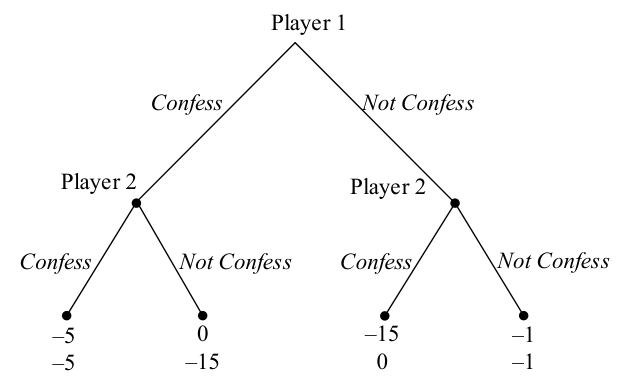
\includegraphics[width=0.55\linewidth]{figures/munoz-garcia-4-3.png}\\[2pt]
\small\textit{Fig.~4.9} Prisoner's dilemma sequential-move game
\end{center}
\begin{enumerate}[label=(\alph*),leftmargin=2em]
\item Find the best responses of the second mover, for each of the first mover's actions.
\item Find the first mover's equilibrium action and describe the subgame perfect Nash equilibrium of
the game.
\item Does the equilibrium behavior in the sequential-move game differ from its simultaneous-move
version?
\end{enumerate}

\begin{referencia}{``its simultaneous-move version'': Muñoz-Garcia \& Toro-Gonzalez (2019), Ch.~1,
Exercise 5 ``Prisoners' Dilemma Game'', Fig.~1.8, p.~9 [PDF 22]. Matrix rebuilt from the page.}
\jogo{Prisoner 1}{Prisoner 2}{\begin{tabular}{c|c|c|}
\hd{} & \hd{Confess} & \hd{Not confess}\\\cline{2-3}
Confess & -5, -5 & 0, -15\\\cline{2-3}
Not confess & -15, 0 & -1, -1\\\cline{2-3}
\end{tabular}}
\vspace{-6pt}\begin{center}\textit{Fig.~1.8} Normal-form of Prisoners' dilemma game\end{center}
\end{referencia}
\resolespaco

% ---------------------------------------------------------------------------
\exercicio{Playing It Safe}{Exam level}{Tadelis (2013), \emph{Game Theory: An Introduction}, Ch.~8
``Credibility and Sequential Rationality'', Exercise 8.10 ``Playing It Safe'', p.~172 [PDF 191]. No
answer in the book. Reproduced verbatim.}

\rot{8.10}\textbf{Playing It Safe:} Consider the following dynamic game: Player 1 can choose to play
it safe (denote this choice by $S$), in which case both he and player 2 get a payoff of 3 each, or he
can risk playing a game with player 2 (denote this choice by $R$). If he chooses $R$ then they play
the following simultaneous-move game:
\jogo{Player 1}{Player 2}{\begin{tabular}{c|c|c|}
\hd{} & \hd{$A$} & \hd{$B$}\\\cline{2-3}
$C$ & 8, 0 & 0, 2\\\cline{2-3}
$D$ & 6, 6 & 2, 2\\\cline{2-3}
\end{tabular}}
\begin{partes}
\item Draw a game tree that represents this game. How many proper subgames does it have?
\item Are there other game trees that would work? Explain briefly.
\item Construct the matrix representation of the normal form of this dynamic game.
\item Find all the Nash and subgame-perfect equilibria of the dynamic game.
\end{partes}
\resolespaco

% ---------------------------------------------------------------------------
\exercicio{Junk Mail Advertising}{Exam level}{Tadelis (2013), \emph{Game Theory: An Introduction},
Ch.~8 ``Credibility and Sequential Rationality'', Exercise 8.13 ``Junk Mail Advertising'',
pp.~173--174 [PDF 192--193]. No answer in the book. Reproduced verbatim.}

\rot{8.13}\textbf{Junk Mail Advertising:} Suppose a single good is owned by a single seller who
values it at $c > 0$ (he can consume the good and get a payoff of $c$). There is a single buyer who
has a small transportation cost $k > 0$ to get to and back from the seller's store, and he values
the good at $v > c + k$. The buyer first decides whether to make the commute or stay at home, not
buy the good, and receive a payoff of 0. If the buyer commutes to the store, the seller can then make
the buyer a take-it-or-leave-it price offer $p \ge 0$. The buyer can then accept the offer, pay $p$,
and get the good, or he can walk out and not buy the good. Assume that $c$, $v$, and $k$ are common
knowledge.
\begin{partes}
\item As best you can, draw the extensive form of this game. What is the best response of the buyer
at the node at which he decides whether to accept or reject the seller's offer?
\item Find the subgame-perfect equilibrium of the game and show that it is unique. Is it Pareto
optimal?
\item Are there Nash equilibria that yield a higher payoff to both players as compared to the
subgame-perfect equilibrium you found in (b)?
\item Now assume that before the game is played the seller can, at a small cost
$\varepsilon < (v - c - k)$, send the buyer a postcard that commits the seller to a certain price
at which the buyer can buy the good (e.g., ``bring this coupon and get the good at a price $p$'').
Would the seller choose to do so? Justify your answer with an equilibrium analysis.
\end{partes}
\resolespaco

% ---------------------------------------------------------------------------
\exercicio{Stackelberg Competition with 2, or 3 Firms}{Exam level}{Muñoz-Garcia \& Toro-Gonzalez
(2019), \emph{Strategy and Game Theory: Practice Exercises with Answers}, 2nd ed., Ch.~4
``Sequential-Move Games with Complete Information'', Exercise 12 ``Stackelberg Competition with 2,
or 3 Firms''$^{\mathrm{B}}$, pp.~185--186 [PDF 197--198]. Worked answer in the book, right after the
statement. Reproduced verbatim (statement only).}

Consider a Stackelberg model of output competition where firm 1 is the industry leader and firm 2 is
the follower. Firms face a linear inverse demand curve $p(Q) = 10 - Q$, where $Q = q_1 + q_2$
denotes the aggregate output sold by both firms. In addition, consider that firms are cost
symmetric, facing a common marginal cost of $MC_i = 2$ for every firm $i = \{1, 2\}$ and no fixed
costs.
\begin{enumerate}[label=(\alph*),leftmargin=2em]
\item Find the equilibrium in this Stackelberg game.
\item Assume now that a new firm (firm 3) joins the industry, acting last (after firm 2 chooses its
output). Find the equilibrium in this Stackelberg game. Compare your results with those in part
(a). How is the output of firm 1 and 2 affected by firm 3's entry?
\end{enumerate}
\resolespaco

% ---------------------------------------------------------------------------
\exercicio{The Rotten Kid Theorem}{Advanced}{Gibbons (1992), \emph{Game Theory for Applied
Economists}, Ch.~2 ``Dynamic Games of Complete Information'', \S2.6 Problems (Section 2.1),
Problem 2.1, p.~130 [PDF 137]. No answer in the book. Reproduced verbatim.}

\rot{2.1.}Suppose a parent and child play the following game, first analyzed by Becker (1974).
First, the child takes an action, $A$, that produces income for the child, $I_C(A)$, and income for
the parent, $I_P(A)$. (Think of $I_C(A)$ as the child's income net of any costs of the action $A$.)
Second, the parent observes the incomes $I_C$ and $I_P$ and then chooses a bequest, $B$, to leave to
the child. The child's payoff is $U(I_C + B)$; the parent's is $V(I_P - B) + kU(I_C + B)$, where
$k > 0$ reflects the parent's concern for the child's well-being. Assume that: the action is a
nonnegative number, $A \ge 0$; the income functions $I_C(A)$ and $I_P(A)$ are strictly concave and
are maximized at $A_C > 0$ and $A_P > 0$, respectively; the bequest $B$ can be positive or negative;
and the utility functions $U$ and $V$ are increasing and strictly concave. Prove the ``Rotten Kid''
Theorem: in the backwards-induction outcome, the child chooses the action that maximizes the
family's aggregate income, $I_C(A) + I_P(A)$, even though only the parent's payoff exhibits
altruism.
\resolespaco

\newpage
% =============================================================================
\bloco{4}{Multistage games and bargaining}{Lecture 4}

% ---------------------------------------------------------------------------
\exercicio{Multistage Practice}{Foundations}{Tadelis (2013), \emph{Game Theory: An Introduction},
Ch.~9 ``Multistage Games'', Exercise 9.1 ``Multistage Practice'', pp.~186--187 [PDF 205--206]. No
answer in the book. Reproduced verbatim.}

\rot{9.1}\textbf{Multistage Practice:} Consider the following simultaneous-move game that is played
twice (the players observe the first-period outcome prior to the second-period play):
\jogo{Player 1}{Player 2}{\begin{tabular}{c|c|c|c|}
\hd{} & \hd{$L$} & \hd{$C$} & \hd{$R$}\\\cline{2-4}
$T$ & 10, 10 & 2, 12 & 0, 13\\\cline{2-4}
$M$ & 12, 2 & 5, 5 & 0, 0\\\cline{2-4}
$B$ & 13, 0 & 0, 0 & 1, 1\\\cline{2-4}
\end{tabular}}
\begin{partes}
\item Find all the pure-strategy subgame-perfect equilibria with no discounting ($\delta = 1$). Be
precise in defining history-contingent strategies for both players.
\item For each of the equilibria you found in (a), find the smallest discount factor that supports
it.
\end{partes}
\resolespaco

% ---------------------------------------------------------------------------
\exercicio{One leader, two followers}{Foundations}{Gibbons (1992), \emph{Game Theory for Applied
Economists}, Ch.~2 ``Dynamic Games of Complete Information'', \S2.6 Problems (Section 2.2), Problem
2.6, p.~133 [PDF 140]. No answer in the book. Reproduced verbatim.}

\rot{2.6.}Three oligopolists operate in a market with inverse demand given by $P(Q) = a - Q$, where
$Q = q_1 + q_2 + q_3$ and $q_i$ is the quantity produced by firm $i$. Each firm has a constant
marginal cost of production, $c$, and no fixed cost. The firms choose their quantities as follows:
(1) firm 1 chooses $q_1 \ge 0$; (2) firms 2 and 3 observe $q_1$ and then simultaneously choose $q_2$
and $q_3$, respectively. What is the subgame-perfect outcome?
\resolespaco

% ---------------------------------------------------------------------------
\exercicio{Online Gaming}{Exam level}{Tadelis (2013), \emph{Game Theory: An Introduction}, Ch.~9
``Multistage Games'', Exercise 9.4 ``Online Gaming'', p.~188 [PDF 207]. No answer in the book.
Reproduced verbatim.}

\rot{9.4}\textbf{Online Gaming:} Consider a two-stage game between two firms that produce online
games. In the first stage, they play a Cournot competition game (each chooses a quantity $q_i$) with
demand function $p = 100 - q$ and zero marginal production costs ($c_i(q_i) = 0$ for $i = 1, 2$).
In the second stage, after observing the pair $(q_1, q_2)$ and after profits have been distributed,
the players play a simultaneous-move ``access'' game in which each can open its platform to allow
players on the other platform to play online with players on its platform ($O$ for player 1, $o$
for player 2), or choose to keep its platform noncompatible ($N$ for player 1, $n$ for player 2), in
which case each platform's players can play only with others on the same platform. If they choose
$(N, n)$ then second-stage payoffs are $(0, 0)$. If only one firm chooses to open its platform, it
bears a cost of $-10$ with no benefit, since the other firm did not allow open access. Finally if
both firms choose $(O, o)$ then each firm gets many more eyeballs for advertising, and payoffs for
each are 2500. Both players use the same discount factor $\delta$ to discount future payoffs.
\begin{partes}
\item Find the unique Nash equilibrium in the first-stage Cournot game and all of the pure-strategy
Nash equilibria of the second-stage access game. Find all the pure-strategy subgame-perfect
equilibria with extreme discounting ($\delta = 0$). Be precise in defining history-contingent
strategies for both players.
\item Now let $\delta = 1$. Find a subgame-perfect equilibrium for the two-stage game in which the
players choose the monopoly (total profit--maximizing) quantities and split them equally (a
symmetric equilibrium).
\item What is the lowest value of $\delta$ for which the subgame-perfect equilibrium you found in
(b) survives?
\item Now let $\delta = 0.4$. Can you support a subgame-perfect equilibrium for the two-stage game in
which the players choose the monopoly quantities and split them equally? If not, what are the
highest profits that the firms can make in a symmetric equilibrium?
\end{partes}
\resolespaco

% ---------------------------------------------------------------------------
\exercicio{Holdup}{Exam level}{Tadelis (2013), \emph{Game Theory: An Introduction}, Ch.~11
``Strategic Bargaining'', Exercise 11.2 ``Holdup'', p.~236 [PDF 255]. No answer in the book.
Reproduced verbatim.}

\rot{11.2}\textbf{Holdup:} Consider an ultimatum game ($T = 1$ bargaining game) in which before
player 1 makes his offer to player 2, player 2 can invest in the size of the pie. If player 2 chooses
a low level of investment ($L$) then the size of the pie is small, equal to $v_L$, while if player 2
chooses a high level of investment ($H$) then the size of the pie is large, equal to $v_H$. The cost
to player 2 of choosing $L$ is $c_L$, while the cost of choosing $H$ is $c_H$. Assume that
$v_H > v_L > 0$, $c_H > c_L > 0$, and $v_H - c_H > v_L - c_L$.
\begin{partes}
\item What is the unique subgame-perfect equilibrium of this game? Is it Pareto optimal?
\item Can you find a Nash equilibrium of the game that results in an outcome that is better for both
players as compared to the unique subgame-perfect equilibrium?
\end{partes}

\begin{referencia}{``ultimatum game ($T = 1$ bargaining game)'': Tadelis (2013), Ch.~11, the first
round of the bargaining game, p.~221 [PDF 240], and \S11.1 ``One Round of Bargaining: The Ultimatum
Game'', p.~222 [PDF 241]. Reproduced verbatim (excerpts).}
In the first round:
\begin{itemize}[leftmargin=1.6em]
\item Player 1 offers shares $(x, 1 - x)$, where player 1 receives $x$ and player 2 receives $1 - x$.
\item Player 2 then chooses to accept, causing the game to end with payoffs $v_1 = x$ and
$v_2 = 1 - x$, or reject, causing the game to move to the second round.
\end{itemize}
[\ldots] We begin the analysis with an easy case in which there is only one round of bargaining, so
that $T = 1$. This is often referred to in the literature as an ultimatum game: player 1 makes an
ultimatum take-it-or-leave-it offer to player 2, and player 2 either accepts it, in which case the
pie is split between the players, or rejects it, in which case both players receive a payoff of
zero.
\end{referencia}
\resolespaco

% ---------------------------------------------------------------------------
\exercicio{Asymmetric Patience 1}{Exam level}{Tadelis (2013), \emph{Game Theory: An Introduction},
Ch.~11 ``Strategic Bargaining'', Exercise 11.5 ``Asymmetric Patience 1'', pp.~236--237 [PDF
255--256]. No answer in the book. Reproduced verbatim.}

\rot{11.5}\textbf{Asymmetric Patience 1:} Consider a three-period sequential (alternating-offer)
bargaining model in which two players have to split a pie worth 1 (starting with player 1 making
the offer). Now the players have different discount factors, $\delta_1$ and $\delta_2$.
\begin{partes}
\item Compute the outcome of the unique subgame-perfect equilibrium.
\item Show that when $\delta_1 = \delta_2$ player 1 has an advantage.
\item What conditions on $\delta_1$ and $\delta_2$ give player 2 an advantage? Why?
\end{partes}

\begin{referencia}{the alternating-offer bargaining model this exercise modifies (``Now the
players have different discount factors''): Tadelis (2013), Ch.~11 ``Strategic Bargaining'',
p.~221 [PDF 240]. Reproduced verbatim (excerpts); with $\delta_1 \neq \delta_2$, player $i$
discounts with $\delta_i$.}
In the first round:
\begin{itemize}[leftmargin=1.6em]
\item Player 1 offers shares $(x, 1 - x)$, where player 1 receives $x$ and player 2 receives $1 - x$.
\item Player 2 then chooses to accept, causing the game to end with payoffs $v_1 = x$ and
$v_2 = 1 - x$, or reject, causing the game to move to the second round.
\end{itemize}
In the second round:
\begin{itemize}[leftmargin=1.6em]
\item A share $1 - \delta$ of the pie is dissipated (the pie is discounted with discount factor
$0 < \delta < 1$).
\item Player 2 offers shares $(x, 1 - x)$, where player 1 receives $x$ and player 2 receives $1 - x$.
\item Player 1 chooses to accept, causing the game to end with payoffs $v_1 = \delta x$ and
$v_2 = \delta(1 - x)$, or reject, causing the game to move to the third round.
\end{itemize}
In the third round and beyond:
\begin{itemize}[leftmargin=1.6em]
\item The game continues in the same way, where following rejection in an odd period player 2 gets
to offer in the next even period, and vice versa.
\item Each period has further discounting of the pie, so that in period $t$ the total pie is worth
$\delta^{t-1}$.
\end{itemize}
[\ldots] Assume for now that the game ends in some prespecified final period $T$, which will be
reached if the players did not reach an agreement in the $T - 1$ periods that preceded $T$.
Furthermore assume that period $T$ is a ``hard deadline,'' so that both players receive a payoff of
zero if they fail to reach an agreement in this last period.
\end{referencia}
\resolespaco

% ---------------------------------------------------------------------------
\needspace{20\baselineskip}
\exercicio{Infinite-Horizon Bargaining Game Between Three Players}{Advanced}{Muñoz-Garcia \&
Toro-Gonzalez (2019), \emph{Strategy and Game Theory: Practice Exercises with Answers}, 2nd ed.,
Ch.~6 ``Repeated Games and Correlated Equilibria'', Exercise 8 ``Infinite-Horizon Bargaining Game
Between Three Players''$^{\mathrm{C}}$, p.~303 [PDF 314]. Worked answer in the book, right after the
statement. Reproduced verbatim (statement only).}

Consider a three-player variant of Rubinstein's infinite-horizon bargaining game, where players
divide a surplus (pie) of size 1, and the set of possible agreements is
\[
X = \{(x_1, x_2, x_3) \mid x_i \ge 0 \quad \text{for } i = 1, 2, 3 \ \text{ and } \ x_1 + x_2 + x_3 = 1\}.
\]
Players take turns to offer agreements, starting with player 1 in round $t = 0$, and the game ends
when \emph{both} responders accept an offer. If agreement $x$ is reached in round $t$, player $i$'s
utility is given by $\delta^t x_i$, where $\frac{1}{2} < \delta < 1$. Show that, if each player is
restricted to using stationary strategies (in which she makes the same proposal every time she is the
proposer, and uses the same acceptance rule whenever she is a responder), there is a unique subgame
perfect equilibrium outcome. How much does each player receive in equilibrium?
\resolespaco

\end{document}

